A continuación se realizará el análisis preliminar de las clases pertenecientes a la zona social del sistema.  Como se ha explicado anteriormente en la sección \nameref{identificacion_subsistemas} perteneciente al capítulo \ref{chapter04}, la zona social engloba los subsistemas de:
\begin{itemize}
	\item gestión de usuarios
	\item gestión de debates
	\item gestión de eventos
	\item gestión de noticias
	\item gestión de entradas del blog
	\item gestión de comentarios
\end{itemize}

La figura \ref{fig:clases_preliminares_modelo_debate} muestra el diagrama de las clases preliminares de la zona social.

\begin{landscape}
	\begin{figure}[ht]
		\centering
		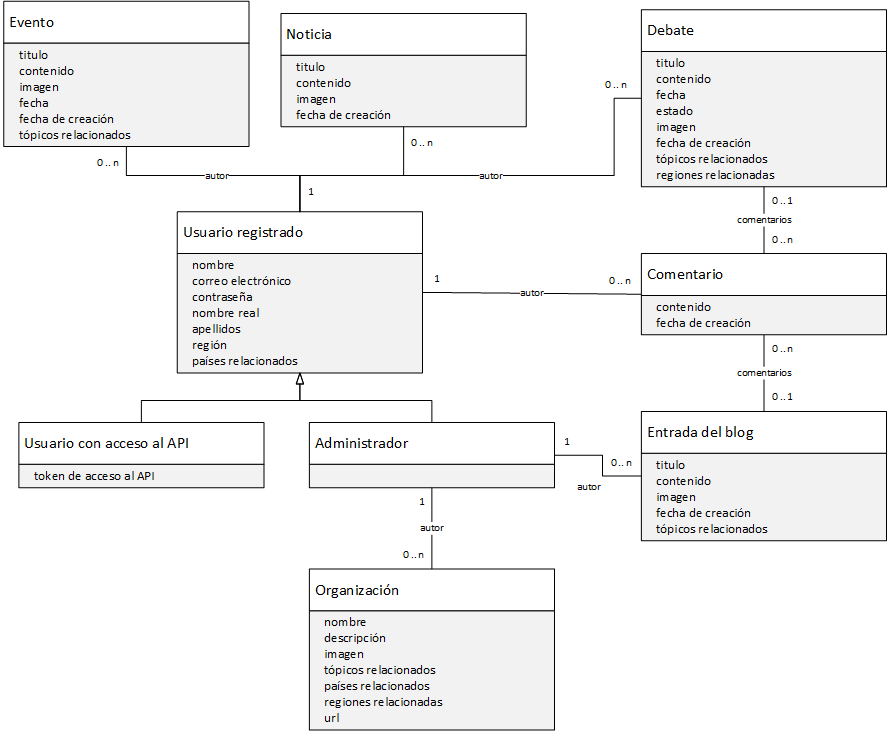
\includegraphics[]{clases/clases_debate_preliminar}
		\caption{Diagrama de clases preliminares de la zona social}
		\label{fig:clases_preliminares_modelo_debate}
	\end{figure}
\end{landscape}

\subsubsection{Descripción de las clases}
\begin{description}
\item[Usuario registrado]	Representa a los usuarios que tienen una cuenta de usuario y han iniciado sesión en el portal.  Puede crear noticias, eventos, debates y realizar comentarios.  Sus atributos son los siguientes:
							\begin{itemize}
								\item \textbf{Nombre}  Será el nombre con el que el sistema identifica a cada usuario.  El nombre de usuario debe ser único.
								\item \textbf{Correo electrónico}  Será la dirección a la que el sistema enviará los correos electrónicos de contacto, por ejemplo: cuando el usuario solicita una nueva contraseña.  El correo electrónico debe ser único.
								\item \textbf{Contraseña}  Será utilizada para autenticar la identidad del usuario al iniciar sesión en el sistema o al modificar la información de su perfil.
								\item \textbf{Nombre real}  Será el nombre real del usuario, podrá ser visto por otros usuarios al visitar su perfil.
								\item \textbf{Apellidos}  Serán los apellidos reales del usuario, podrán ser vistos por otros usuarios al visitar su perfil.
								\item \textbf{Continente}  Será el continente en el que se encuentra el usuario.  Éste atributo no será obligatorio y podrá estar vacío.
								\item \textbf{Países relacionados}  Serán los países en los que el usuario tiene algún tipo de interés.  Este atributo no será obligatorio y podrá estar vacío.
							\end{itemize}
\item[Usuario con acceso al API]  Representa a los usuarios registrados que tienen capacidad de acceso al API del sistema.  Tienen las mismas capacidades que cualquier usuario registrado.  Además de los atributos de cualquier usuario registrado también tendrán:
							\begin{itemize}
							\item \textbf{Token}  Será la clave con la que el usuario accede al API.  Ésta clave será secreta y no podrá ser vista por ningún otro usuario.
							\end{itemize}
\item[Administrador]  Representa a los usuarios registrados con privilegios de administración en el sistema.  Tendrán los mismos atributos que cualquier otro usuario registrado pero podrán crear, modificar y eliminar cualquier contenido o comentario.
\item[Noticia]  Representa una noticia de interés en la que la fecha no es importante.  Las noticias podrán ser creadas por cualquier usuario registrado.  Sus atributos serán los siguientes:
							\begin{itemize}
							\item \textbf{Título}  Es el título de la noticia.
							\item \textbf{Contenido}  Es el contenido de la noticia.
							\item \textbf{Imagen}  Es una imagen relacionada con el contenido de la noticia.  Éste atributo no será obligatorio y podrá estar vacío.
							\item \textbf{Fecha de creación}  Es la fecha en la que la noticia fue creada.  Este campo es almacenado automáticamente por el sistema.
							\item \textbf{Autor}  Es el usuario registrado que crea la noticia.  Cada noticia tendrá un único autor, pero cada usuario registrado podrá ser autor de múltiples noticias.
							\end{itemize}
\item[Evento]  Representa una situación o noticia que tendrá lugar en un determinado momento del tiempo.  Los eventos podrán ser creados por cualquier usuario registrado.  Sus atributos serán los siguientes:
							\begin{itemize}
							\item \textbf{Título}  Es el título del evento.
							\item \textbf{Contenido}  Es el contenido del evento, donde se explica toda la información necesaria.
							\item \textbf{Imagen}  Es una imagen relacionada con el contenido del evento.  Éste atributo no será obligatorio y podrá estar vacío.
							\item \textbf{Fecha}  Será la fecha en la que el evento tendrá lugar.
							\item \textbf{Fecha de creación}  Es la fecha en la que el evento fue creado.  Este campo es almacenado automáticamente por el sistema.
							\item \textbf{Tópicos relacionados}  Serán los tópicos relacionados con el contenido del evento.  Los tópicos servirán como metainformación sobre el contenido y ayudarán a enriquecer los resultados de la búsqueda.
							\item \textbf{Autor}  Es el usuario registrado que crea el evento.  Cada evento tendrá un único autor, pero cada usuario registrado podrá ser autor de múltiples eventos.
							\end{itemize}
\item[Debate]  Representa un tema u opinión en el que se quiere permitir la participación de los usuarios.  Sus atributos serán los siguientes:
							\begin{itemize}
							\item \textbf{Título}  Es el título del debate.
							\item \textbf{Contenido}  Es el contenido del debate, donde se expone el tema a tratar por los usuarios.
							\item \textbf{Fecha}  Será la fecha o periodo de fechas en las que el debate tendrá lugar.
							\item \textbf{Estado}  Es el estado en el que se encuentra el debate.  Los posibles estados son ``abierto'', ``cerrado'' o ``próximamente''.
							\item \textbf{Imagen}  Es una imagen relacionada con el contenido del debate.  Éste atributo no será obligatorio y podrá estar vacío.
							\item \textbf{Fecha de creación}  Es la fecha en la que el debate fue creado.  Este campo es almacenado automáticamente por el sistema.
							\item \textbf{Tópicos relacionados}  Serán los tópicos relacionados con el contenido del debate.  Los tópicos servirán como metainformación sobre el contenido y ayudarán a enriquecer los resultados de la búsqueda.
							\item \textbf{Regiones relacionadas}  Serán las regiones relacionadas con el debate o a las que éste hace referencia.  Al igual que los tópicos, las regiones servirán como metainformación sobre el contenido y ayudarán a enriquecer los resultados de la búsqueda.
							\item \textbf{Autor}  Es el usuario registrado que crea el debate.  Cada debate tendrá un único autor, pero cada usuario registrado podrá ser autor de múltiples debates.
							\item \textbf{Comentarios}  Son los comentarios que los usuarios realizan en el debate.  Cada debate podrá tener múltiples comentarios, pero cada comentario sólo podrá pertenecer a un debate.
							\end{itemize}
\item[Entrada del blog]  Representa una entrada en el blog oficial de Land Portal.  Las entradas en el blog sólo pueden ser creadas por los administadores.  Sus atributos son los siguientes:
							\begin{itemize}
							\item \textbf{Título}  Es el título de la entrada.
							\item \textbf{Contenido}  Es el contenido de la entrada.
							\item \textbf{Imagen}  Es una imagen relacionada con el contenido de la entrada.  Éste atributo no será obligatorio y podrá estar vacío.
							\item \textbf{Fecha de creación}  Es la fecha en la que la entrada fue creada.  Este campo es almacenado automáticamente por el sistema.
							\item \textbf{Tópicos relacionados}  Serán los tópicos relacionados con el contenido de la entrada.  Los tópicos servirán como metainformación sobre el contenido y ayudarán a enriquecer los resultados de la búsqueda.
							\item \textbf{Autor}  Es el administrador que crea la entrada.  Cada entrada tendrá un único autor, pero cada administrador podrá ser autor de múltiples entradas.
							\item \textbf{Comentarios}  Son los comentarios que los usuarios realizan en la entrada.  Cada entrada podrá tener múltiples comentarios, pero cada comentario sólo podrá pertenecer a una entrada.
							\end{itemize}
\item[Comentario]  Representa la opinión que un usuario hace pública en un debate o una entrada del blog:
							\begin{itemize}
							\item \textbf{Contenido}  Es el contenido del comentario.
							\item \textbf{Fecha de creación}  Es la fecha en la que el comentario fue creado.  Este campo es almacenado automáticamente por el sistema.
							\item \textbf{Autor}  Es el usuario registrado que crea el comentario.  Cada comentario tiene un autor, pero un usuario registrado puede ser autor de múltiples comentarios.
							\end{itemize}
\end{description}